\documentclass{article}

\usepackage{Sweave}
\begin{document}
\Sconcordance{concordance:testingPDF.tex:testingPDF.Rnw:%
1 2 1 1 0 2 1 1 2 1 0 1 3 2 0 1 1 6 0 1 5 10 0 1 2 5 0 1 2 3 1}


\begin{Schunk}
\begin{Sinput}
> ndata <- read.csv("AAPL SPX 10Y OiL - Copy.csv")
> # SUPER usefull function of attach, which makes easier to give just the names 
> #from the data file
> attach(ndata)
> str(data)
\end{Sinput}
\begin{Soutput}
function (..., list = character(), package = NULL, lib.loc = NULL, verbose = getOption("verbose"), 
    envir = .GlobalEnv)  
\end{Soutput}
\begin{Sinput}
> #data$Date <- as.Date(Date,format="%m/%d/%Y")
> #Vardan: Create a new column with id
> #id<-seq(1,261,by=1)
> #data<-data.frame(id,Date,aapl,spx,X10y,wti)
> str(data)
\end{Sinput}
\begin{Soutput}
function (..., list = character(), package = NULL, lib.loc = NULL, verbose = getOption("verbose"), 
    envir = .GlobalEnv)  
\end{Soutput}
\begin{Sinput}
> #data<- data[order(id, decreasing = TRUE),]
> plot(spx)
\end{Sinput}
\end{Schunk}
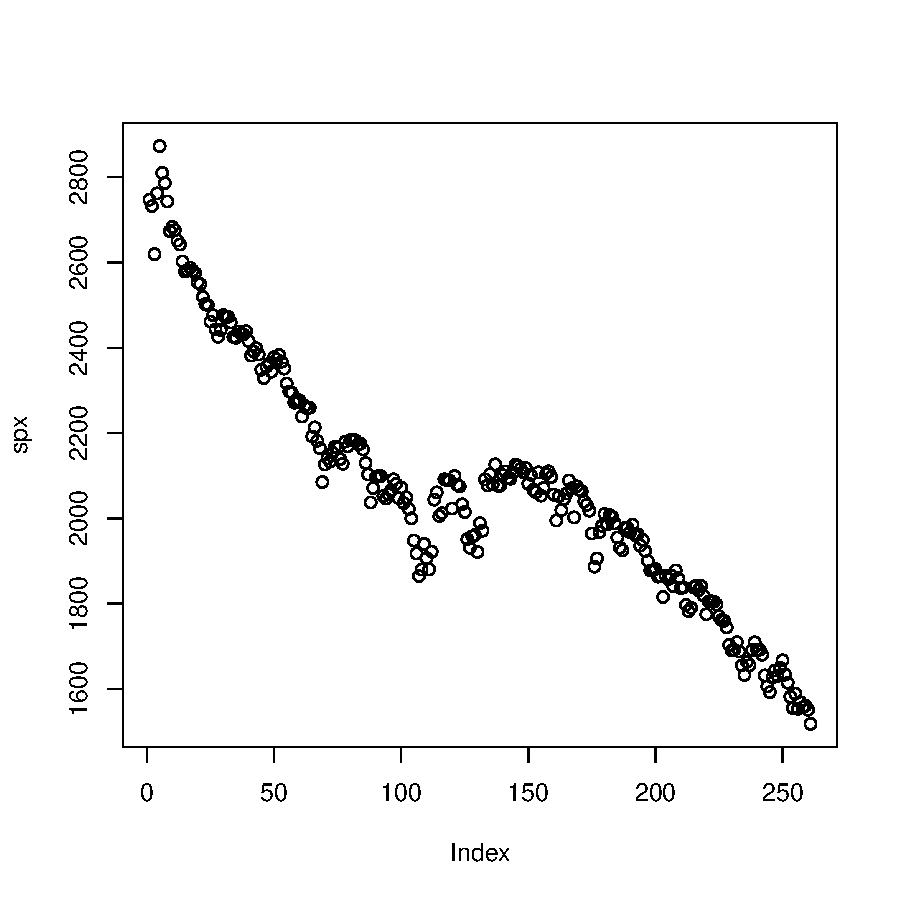
\includegraphics{testingPDF-001}



\end{document}
